\section{Results}
\label{sec:results}

All intervals are nominal 95\% Wald intervals. Coverage is reported with Monte Carlo standard errors of about $0.01$ at $R=\REPSSYN$ and $0.013$ at $R=\REPSREAL$. Width ratios are relative to PPI++ on the same replications, with the same labeled and unlabeled samples. The efficient bound is the asymptotic width ratio of the oracle calibrator for the information used (for \emph{f}-only pools it is $\sqrt{V^\star(f)/V_{\rm PPI++}}$, and for pools with covariates the same with $(f,X)$ against PPI++ with linear covariate adjustment).

\subsection{Synthetic data with known truth}

\cref{fig:synth} plots the width ratio against labeled size $n$ at $N=4n$. Each panel is one scenario. Under \emph{linear calibration}, $m$ is affine in $f$, and the bound is 1: no method beats PPI++, and the flexible calibrators widen intervals by $16\%$ at $n=50$ (spline) and $19\%$ (boosting), shrinking to $1\%$ at $n=1000$. This is the predicted cost $(1-a)\mathrm{Var}(\hat m-m)/n$ with $\hat m$ estimated from few labels.

Under \emph{nonlinear calibration}, the spline calibrator gives width ratios $0.83$, $0.81$ and $0.82$ at $n=50,200,1000$, against a bound of $0.756$. The gap to the bound is the learner's own error, which is consistent with the theory: the realized gain is the bound's gain minus $(1-a)\mathrm{Var}(\hat m-m)/n$. Boosting is slightly better at $n\ge200$ ($0.77$--$0.80$) and also narrower at $n=50$ ($0.86$). The stratified PPI estimator of \citet{fisch2024strat} does not gain in this scenario (ratio $0.99$--$1.00$); its piecewise-constant calibrator has a larger error than the spline. \emph{Binary} outcomes give a small bound (0.98) and small gains at $n\ge200$. \emph{Covariates beyond $f$} make PPI++ on $f$ alone inefficient through $E(m_X-m_f)^2$: the spline with covariates reaches $0.82$ against a bound of $0.76$. \emph{Heavy-tailed} noise gives 0.88--0.90 against a bound of 0.86, with coverage unaffected.

Coverage is between $0.92$ and $0.97$ for PPI, PPI++ and the cross-fitted estimators in every cell, with no systematic difference between them. Stratified PPI is the exception: its coverage falls to $0.91$ in several small-sample cells (for example, $n=50$ with $N=4n$ under the binary and heavy-tailed scenarios), where the estimated stratum weights and small per-stratum samples make the linearized variance too small.

\begin{figure*}[t]
  \centering
  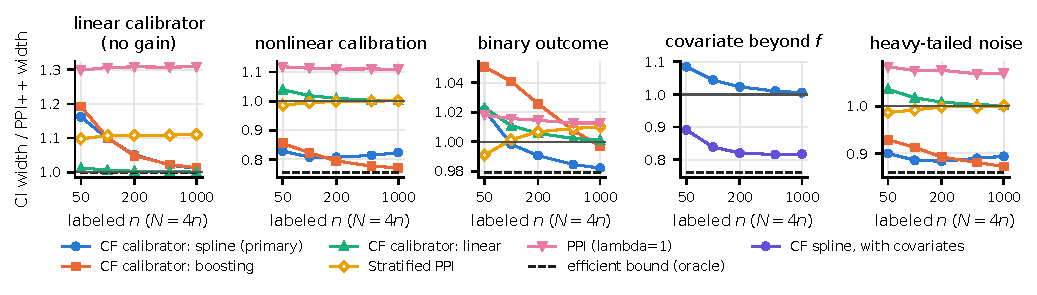
\includegraphics[width=\textwidth]{figures/fig_synth.pdf}
  \caption{Synthetic data, $N=4n$, 500 replications per point. The vertical axis is the mean CI width relative to PPI++ on the same samples. Dashed: efficient bound for the information used (oracle calibrator). Points above 1 are wider than PPI++.}
  \label{fig:synth}
\end{figure*}

\subsection{Agreement with the variance formulas}

To test the formulas without learner noise, \cref{tab:theory} (appendix) compares Monte Carlo standard deviations and width ratios with the predictions of \cref{prop:var} for oracle calibrators with error variance $s^2\in\{0,0.04\}$ and $\{0,0.16\}$. Across the five scenarios, three values of $\mathrm{Var}(\hat m-m)$, $n\in\{50,200,1000\}$ and $N/n\in\{1,4,16\}$, the width ratios agree with the prediction to within $2\%$ (largest discrepancy $1.7\%$, nonlinear scenario), and the Monte Carlo standard deviations agree to within $1\%$ (median) except one case: the heavy-tailed scenario at $n=1000$, where the predicted SD is $9\%$ too small. We attribute this to the slow convergence of the Monte Carlo estimate of the population variance of $t_3$ noise (its fourth moment is infinite); we did not verify this directly. These checks hold for the bound itself (e.g., $0.757$ observed against $0.756$ predicted in the nonlinear case).

\subsection{Public pools with exact coverage checks}

We use the seven pools that have labels and predictions for every unit (\cref{sec:exp}). \cref{tab:real} reports, for each pool and information set, the efficient-bound ratio at $N=4n$ (computed from the pool-level constants with the formula in \cref{cor:when}) and the realized width ratio of the spline calibrator at $n=50,200,1000$. \cref{fig:real} shows the realized ratios at $n=200$ for all calibrators.

The bound is between $0.98$ and $1.00$ for every pool and information set. The estimated nonlinear shares $\kappa=\Delta_L/\mathbb E(Y-L)^2$ are $0.2\%$ to $5.4\%$ (\cref{tab:pool}, appendix). Forest, alphafold and gene expression have the largest shares and the largest possible gains. Realized gains are absent. At $n=50$ the spline calibrator is $5$--$11\%$ wider than PPI++; at $n=200$ it is $1$--$4\%$ wider; at $n=1000$ it is within $1\%$. The boosting calibrator is wider still ($2$--$9\%$ at $n=200$), and the linear calibrator is within $2\%$ of PPI++ at $n=200$. Adding covariates to PPI++ changes width by less than $1\%$ at $n\ge200$ on these pools.

PPI++ itself does shorten intervals substantially relative to the labeled-only mean: classical intervals are $1.14$--$1.98$ times wider than PPI++ at every $n$ we tried (\cref{tab:realsens} reports $n=200$). The pools therefore confirm the value of prediction-powered inference, but not of further flexibility.

Coverage at the nominal level holds for all methods on all pools. Per-cell coverage is between $0.89$ and $0.98$ for $n\ge200$, with the lowest values on census income. At $n=50$, census income undercovers for every method, PPI++ and the classical mean included: coverage is $0.83$--$0.89$. The heavy right tail of the income outcome makes the normal approximation poor at this size. Forest at $n=50$ over-covers ($0.96$--$0.97$) because the outcome is discrete.

\begin{table*}[t]
  \centering
  \caption{Public pools (exact coverage checks, $N=4n$, \REPSREAL{} replications per cell). \emph{Bound}: efficient-bound width ratio vs PPI++ at $a=1/5$, from pool-level quantities. $n=50,200,1000$: realized width ratio of the spline-calibrated estimator vs PPI++ (with linear covariate adjustment in the $f{+}X$ rows). Coverage columns give the range over all $(n,N/n)$ cells.}
  \label{tab:real}
  \small
  \begin{tabular}{llcccccc}
\toprule
Pool & Info & Bound & $n{=}50$ & $n{=}200$ & $n{=}1000$ & CF cov.\ range & Baseline cov.\ range \\
\midrule
galaxies & f & 0.997 & 1.051 & 1.015 & 1.004 & 0.927--0.963 & 0.923--0.960 \\
forest & f & 0.980 & 1.072 & 1.015 & 1.000 & 0.910--0.970 & 0.913--0.963 \\
gene expr. & f & 0.997 & 1.080 & 1.014 & 1.002 & 0.933--0.973 & 0.927--0.970 \\
alphafold & f & 0.992 & 1.067 & 1.015 & 1.002 & 0.913--0.957 & 0.903--0.963 \\
alphafold & f+X & 0.987 & 1.092 & 1.021 & 1.003 & 0.923--0.967 & 0.897--0.963 \\
census income & f & 0.998 & 1.095 & 1.034 & 1.007 & 0.840--0.953 & 0.833--0.947 \\
census income & f+X & 0.995 & 1.107 & 1.039 & 1.007 & 0.830--0.953 & 0.820--0.957 \\
census health & f & 0.999 & 1.047 & 1.014 & 1.003 & 0.940--0.977 & 0.930--0.970 \\
census health & f+X & 0.999 & 1.053 & 1.015 & 1.004 & 0.917--0.967 & 0.920--0.957 \\
census educ. & f & 0.999 & 1.067 & 1.021 & 1.004 & 0.927--0.973 & 0.910--0.967 \\
census educ. & f+X & 0.998 & 1.105 & 1.035 & 1.008 & 0.917--0.960 & 0.903--0.953 \\
\bottomrule
\end{tabular}

\end{table*}

\begin{figure}[t]
  \centering
  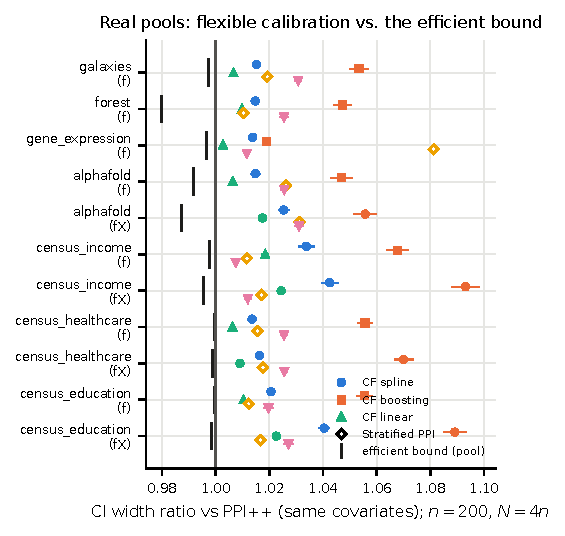
\includegraphics[width=\columnwidth]{figures/fig_real.pdf}
  \caption{Real pools at $n=200$, $N=4n$. Points: realized width ratios vs PPI++ (with covariate adjustment in $f{+}X$ rows) for each calibrator, with 95\% Monte Carlo intervals. Ticks: efficient bound from pool-level quantities.}
  \label{fig:real}
\end{figure}

\subsection{Larger labeled samples}

To test whether the realized gap closes with more labels, we extended four pools that span the range of nonlinear shares to $n=5{,}000$ and $n=20{,}000$ ($N=4n$, 100 replications per cell). The spline calibrator's width ratio moves down toward the bound as $n$ grows: at $n=20{,}000$ it is $0.995$ on \texttt{forest} (bound $0.980$), $0.998$ on \texttt{gene\_expression} (bound $0.997$), $0.998$ on \texttt{alphafold} (bound $0.992$), and $1.000$ on \texttt{census\_education} with covariates (bound $0.998$). Realized gains therefore appear only at the largest sample sizes, and on \texttt{forest} they recover a quarter of the bound's $2\%$. Coverage stays between $0.92$ and $0.96$ for PPI++ and the spline calibrator (100 replications, Monte Carlo standard error about $0.025$).

\subsection{Summary of conditions}

Across the three evidence sources, the width reduction is governed by two quantities that can be estimated from the data at hand: the nonlinear share $\kappa$ of the calibration function (which sets the bound), and the learner's error variance at the available $n$ (which sets the realized gain). A reduction is realized when $\mathrm{Var}(\hat m-m)<\Delta_L$ and only then. Under linear calibration, under small $n$ relative to the complexity of $m$, or under small nonlinear share, PPI++ is the better interval.
